\subsubsection*{The Modelling Problem}

More formally, suppose that we have a mathematical model
$M_{\mathbf{p}}$ parameterised by the vector
$\mathbf{p}\in\mathcal{P}$. For example, $M_{\mathbf{p}}$ may be a
parameterised partial differential equation %(PPDE)
in a storm surge model. For each $\mathbf{p}$ we suppose the model is
well-defined and there exists a unique function
\begin{equation}
  \label{eq:1}
  U_{\mathbf{p}}(\mathbf{x})\, \quad \mathbf{x}\in\Omega
\end{equation}
which is a solution to the model problem, that is $M_{\mathbf{p}}(U_{\mathbf{p}})=0$.
Here the \emph{domain space} $\Omega$ represents variables such as 
time and space, 
and $U_{\mathbf{p}}$ represents scalar or vector fields of interest, 
such as storm surge water level and/or velocity.    

Sometimes the goal of the modeller is to better understand the
relationship between $\mathbf{p}$ and some lower-dimensional quantity
of interest $Q(U_{\mathbf{p}})$, such as the relationship between a
particular rainfall scenario and the maximum storm surge levels at
particular geographical locations. In order to achieve such
understanding, repeated executions of the model (or approximations of the model solution) are often required
with an expert analysis of the outputs of each stage and selection of
the next parameter set based on an assessment of those outputs. Such
repeated model executions can also be used to estimate the
\emph{uncertainty} in any given set of predictions of
$Q(U_{\mathbf{p}})$. Through the process of trying different model
parameterisations, the scientist is able to build up an understanding
of the \emph{general} relationship between $\mathbf{p}$ and
$Q(U_{\mathbf{p}})$, including the areas of the parameter space
$\mathcal{P}$ which have the greatest influence on the result and
which types of uncertainty have the greatest impact on the certainty
of the results.

\paragraph*{A specific storm-surge example:}
Consider the problem of predicting the maximum 
storm surge water level along a coast threatened by a cyclone. 
A mathematical model of storm surge is provided 
by the shallow water wave equation,  which encodes the conservation of water and Newton's second Law (Force = mass $\times$ acceleration) 
\begin{align*}
\frac{\partial h}{\partial t} +
\frac{\partial }{\partial x} \left(uh\right) + \frac{\partial }{\partial y} \left(vh\right) &= R, \\
\frac{\partial uh}{\partial t} +
\frac{\partial }{\partial x} \left(u^2h  \frac12 gh^2 \right) 
+ \frac{\partial }{\partial y} \left(vuh\right) &= gh \frac{\partial b}{\partial x} 
+ \frac{\partial P}{\partial  x} + S_{fx} + S_{wx} ,\\
\frac{\partial vh}{\partial t} +
\frac{\partial }{\partial x} \left(uvh  \right) 
+ \frac{\partial }{\partial y} \left(v^2h + \frac12 g h^2 \right) &= gh \frac{\partial b}{\partial y} 
+ \frac{\partial P}{\partial  y} + S_{fy} + S_{wy},
\end{align*}
where $h(x,y,t)$ is the depth of water, $u(x,y,t)$ and $v(x,y,t)$ are the $x$ and $y$ horizontal components of water velocity, $g$ is the gravitational constant (9.81), $b(x,y)$ is the bathymetry (elevation of the ocean bed), $R$ is the rate of rainfall, $P$ is the atmospheric pressure (which generates a surge due to spatial differences in atmospheric pressure associated with a large cyclone), $S_{fx}$ and $S_{fy}$ are the $x$ and $y$ components of the frictional force generated by the flow of the surge over the ocean bed (flow over sand is different than flow through mangroves) , and $S_{wx}$ and $S_{wy}$ are the $x$ and $y$ components of the surface stress force (generated by the wind). As is evident, there are many opportunities for uncertainty in the data defining this model. 
As demonstrated in our papers~\parencite{anugamanual,nielsen2005hydrodynamic}  these
equations and their implementation in the AnuGA package provide a reliable
model of general flows associated with inundation due to riverine flooding, storm-surge 
and tsunamis.

The parameter space $\mathcal{P}$ needs to represent the variation in the input data $R$, $b$, $P$, $S_f$, $S_w$, as well as design parameters describing actions such as raising or lowering flood barriers and releasing or diverting flow from upstream rivers, or flood basins, or indeed constructing emergency levees. 
The domain $\Omega$ represents the variables $x$, $y$ over a geographical region and $t$ over a time interval, such as a  coastal region threatened by a cyclone over particular time interval. The model solution 
$$
U_{\mathbf{p}} (\mathbf{x})  = \begin{bmatrix} h(x,y,t) \\ u(x,y,t) \\ v(x,y,t) \end{bmatrix}
$$
represents the water depth and velocity fields obtained by solving the model problem for a particular value of the parameter $\mathbf{p}$ (or perhaps a high fidelity numerical approximation of this problem). 

A quantity of interest $Q(U_{\mathbf{p}})$ could be the maximum storm surge height at a particular location $(x_0, y_0)$
$$ 
Q(U_{\mathbf{p}})  = \max_{t_0 \leq t \leq t_1} \left( h(x_0,y_0,t) + b(x_0,y_0) \right).
$$
The aim of  uncertainty quantification is to obtain useful relationships between the variations in pressure, wind and rainfall  and $Q(U_{\mathbf{p}})$, including the which components of the inputs  which have the greatest influence on the result. 




%or to find the parameter choice $\mathbf{p}$
%which optimises $Q$. %over all $\mathbf{x}$.
%This high-level description of the ``model selection/optimisation''
% workflow 
%(shown
%graphically in Figure~\ref{fig:general-fb-loop})
 %lies at the heart of
%a great deal of modern science.
%\begin{figure}
 % \centering
  %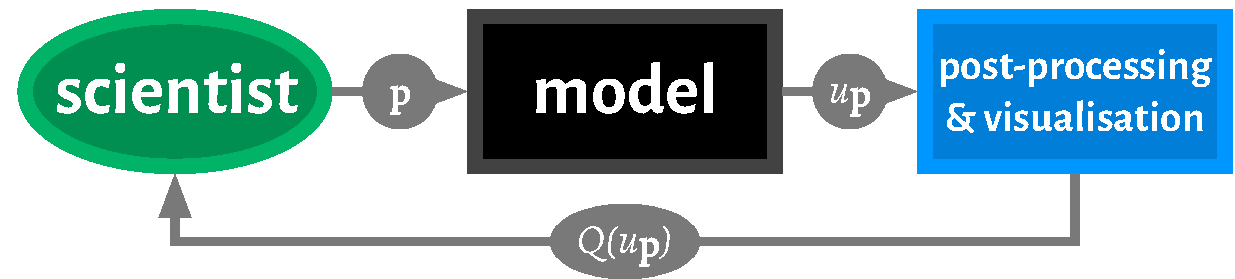
\includegraphics[width=.6\textwidth]{figures/general-fb-loop.pdf}
  %\caption{The human-in-the-loop modelling workflow. A scientist
    %selects an initial parameter $\mathbf{p_0}$ for their model,
    %examines the model output $Q(u_{\mathbf{p}})$, and either accepts
    %the output of the model or re-runs the model with a different
    %choice of the parameter $\mathbf{p_1}$.}
  %\label{fig:general-fb-loop}
%\end{figure}
%There are many ways of finding an optimal $\mathbf{p}$, from 
%trial-and-error experimentation to expert judgement through to fully-automated algorithmic
%optimization procedures. Often there are ways to optimise $\mathbf{p}$
%algorithmically, although these methods often introduce new parameters (the
%arguments of the function being optimised) which must be selected by the
%scientist. 
%As a result, this feedback loop will often require many
%iterations, with a scientist-in-the-loop, evaluating the results
%of the model (possibly through visualising the model output) and
%choosing a parameter update $\Delta\mathbf{p}$ at each step.
% (see
%Figure~\ref{fig:unrolled-fb-loop}). 
%Each step through this loop
%provides feedback to the scientist about the response of the system to
%a particular value of $\mathbf{p}$ --  for example, the maximum storm
%surge level under a particular rainfall scenario. 

%\begin{figure}
% \centering
%  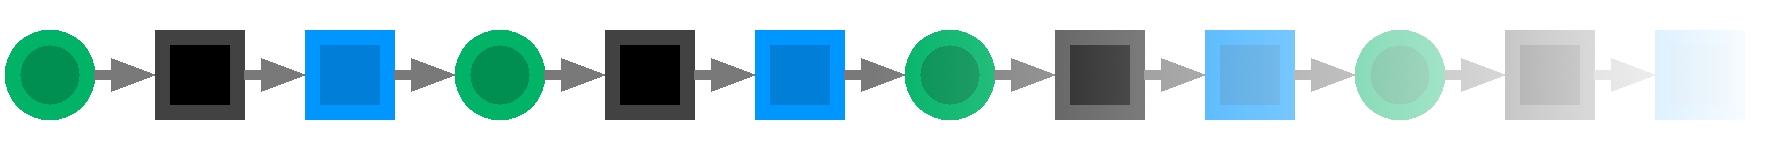
\includegraphics[width=\textwidth]{figures/unrolled-fb-loop.pdf}
%  \caption{If the modelling \& post-processing/visualisation steps can
%    be performed sufficiently quickly, then the scientist can explore
%    the $\mathbf{p} \rightarrow Q(u_{\mathbf{p}})$ relationship
%    \emph{interactively}, with the all the associated benefits for
%    exploratory analysis.}
%  \label{fig:unrolled-fb-loop}
%\end{figure}

From a workflow perspective, the productivity of the
modeller/scientist is proportional to the rate at which they can
explore the $\mathbf{p} \rightarrow Q(U_{\mathbf{p}})$ relationship.
Any latency improvements in this feedback loop will translate into
productivity gains~\parencite{liuEffects2014}. If the model
parameters $\mathbf{p}$ and inputs $\mathbf{x}$ are known precisely
and the quantity $Q(U_{\mathbf{p}})$ is cheap to calculate and easy to
interpret, then the task is simple: provide the scientist with an
interface for manipulating $\mathbf{p}$ and set them loose. However,
for real-world models (such as those used in flood/storm
surge/bushfire modelling) this is often not the case. There are
\textbf{three primary challenges}:
\begin{enumerate}
\item \emph{The model may not provide a way to express uncertainty in
    the inputs}. Many models do not provide methods for including
  uncertainty information in their inputs, as was the case in the 2011
  Brisbane River flood example.
\item \emph{The quantity $Q(U_{\mathbf{p}})$ may not be cheap to
    calculate}. Many
  sophisticated models require non-trivial computing resources 
  to evaluate. These compute resources may be
  difficult to secure, with submitted jobs having to wait in a queue, 
  and may
  take a long time to compute even when the resources are available.
  This is especially problematic in a disaster-response scenario,
  where an approximately correct answer provided in a short time is
  significantly more useful than a perfect answer provided after it is
  too late to act on.
\item \emph{The quantity $Q(U_{\mathbf{p}})$ together with estimates
    of its uncertainty may not be easy to interpret}. Oftentimes this
  is a visualisation problem--- the mapping
  $\mathbf{p} \rightarrow Q(U_{\mathbf{p}})$ may be high-dimensional,
  and presenting that to a decision-maker, particularly when combining
  it with its uncertainty estimates, may not be straightforward.
\end{enumerate}
%\begin{figure}
 % \centering
  %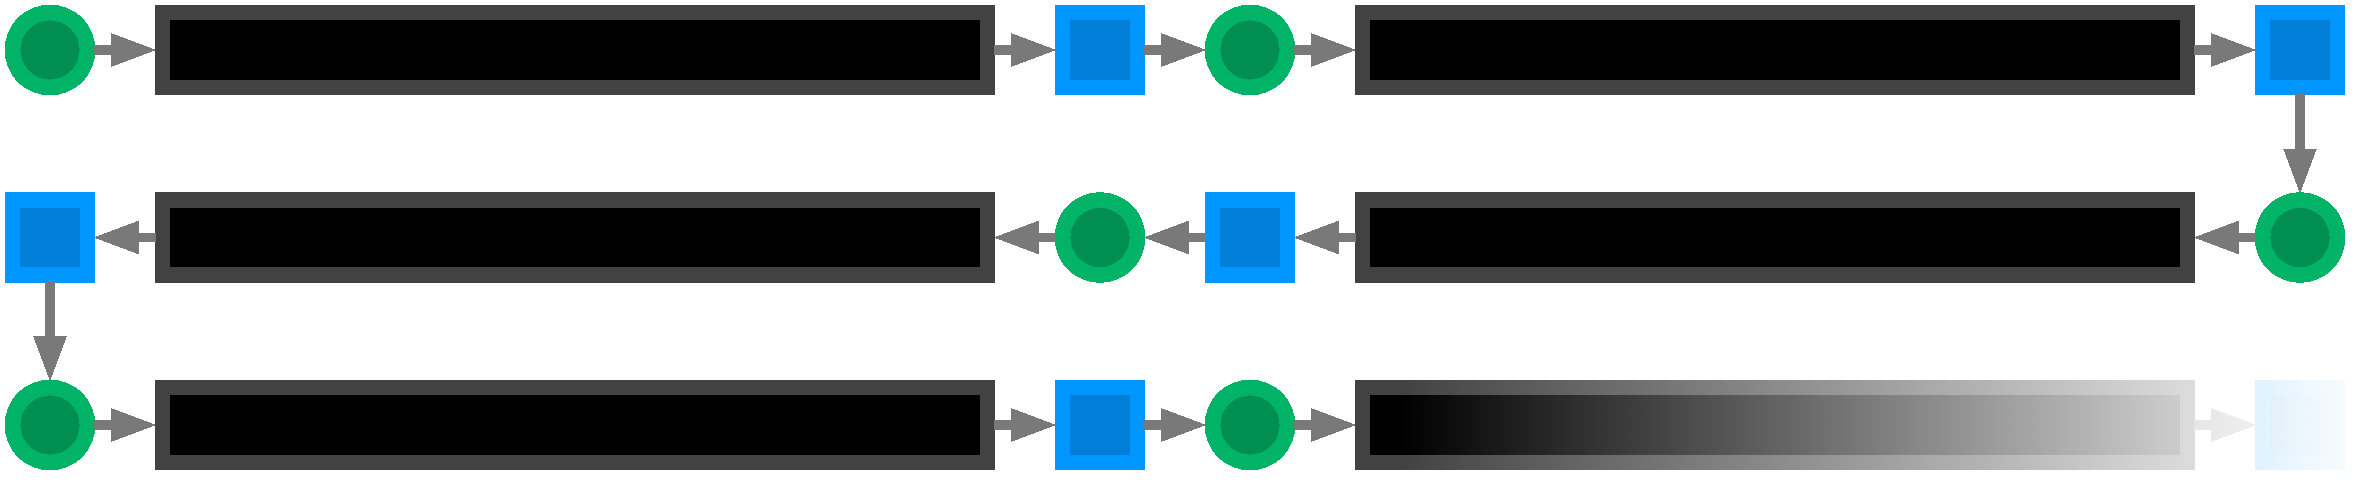
\includegraphics[width=\textwidth]{figures/long-fb-loop.pdf}
  %\caption{If the model is computationally expensive to run, then the
   % workflow is dominated by waiting for the model to finish. This
    %results in lower productivity---not only due to the time spent
    %waiting for the model, but also because of the temporal separation
  %between the selection of a new parameter $\mathbf{p}$, and seeing
 % its impact on the results of the model.}
 % \label{fig:long-fb-loop.pdf}
%\end{figure}

